\section{Mechanism}\label{secmech}
Looking back at model interpretation for random forest, its central spirit is to establish the idea of feature contribution.
By computing label distribution, a measure of the change is then obtained and associated with the split feature.  
In the case of GBDT, we can expand this computation with a slight modification. Because the targets of the latter trees
are the residual, it should replace the instance label while computing label distribution.
Nevertheless, the problem of this version is that the average of labels on a leaf node is not always equal to the score
on it. So the valuable model information in these scores are not utilized and the method is not appropriate for different GBDT 
versions \cite{friedman2001greedy,chen2016xgboost}.

In fact, the loss function determines the optimal coefficient and table \ref{tabloss} shows some common examples.
LS and LAD stand for Least Square and Least Absolute Deviation respectively. $\tilde{y}_{i}$ is the residual updated after
each iteration. $F_{m-1}(x_{i})$ is the approximation on iteration $(m-1)$. $g_{i}$ and $h_{i}$ are the first and second order
gradient statistics on the loss. Different from the numerical optimization essence to compute negative gradient (for LS and LAD), 
XGB\cite{chen2016xgboost} first approximates the loss function with its second order Taylor expansion and an analytic solution is then got.
So it contains no negative gradient computation and the evaluation of leaf weights is far from the label average. 
Particularly,  only if the LS loss function and traditional GBDT training process is used, the  label averages meet the scores.
\begin{table}[htbp]
  \centering
  \caption{Loss Functions of GBDT}
\label{tabloss}
    \begin{tabular}{llll}
     \shline
    Settings    \quad & Loss Function& \quad Negative Gradient& \quad Leaf weight \\
    \hline
     LS&    $\frac{1}{2}[y_{i}-f(x_{i})]^{2}$     &  \quad $y_{i}-f(x_{i})$   &  $\quad ave_{x_{i}\in R_{jm}}{\tilde{y}_{i}}$ \\
     \specialrule{0em}{2pt}{1pt}
     LAD&    $\mid y_{i}-f(x_{i})\mid$   &  $\quad sign[y{}_{i}-f(x_{i})]$     & \tiny $\quad median_{x_{i}\in R_{jm}}{\{y_{i}-F_{m-1}(x_{i})\}}$ \\
     \specialrule{0em}{3pt}{1pt}
   \multirow{2}*{XGB} &   \small $\sum_{i=1}^{n}[l((y_{i},\hat{y}^{(t-1)}))+g_{i}f_{t}(x_{i})$   &     \multirow{2}*{\qquad/}    &  \multirow{2}*{  $\quad -\frac{\sum_{i\in I_{j}}g_{i}}{\sum_{i\in I_{j}}h_{i}+\lambda} $}\\
  &   \small  $+\frac{1}{2}h_{i}f_{t}^{2}(x_{i}))]+\Omega(f_{t})$& & \\
   \shline
    \end{tabular}%
  \label{tab:addlabel}%
\end{table}%

Without loss of generality, the interpretation for GBDT needs to work on the 
leaf scores. Since the scores are only assigned
to leaf nodes, we have to find a way to propagate them back all the way to the root. The left tree of Fig \ref{figgbdt} shows an example
tree in a GBDT model, with split feature and split value marked on arcs. Observing the three nodes in the rounded rectangle, 
the instances in node 6 will get a score difference as: $S_{n11}-S_{n12}=0.085-0.069=0.016$, where $S_{nk}$ is the score on node k. 
Moreover, this difference is caused by splitting feature $feat5$ branching by a threshold of 1.5. We can allocate this difference to the
two branches by assigning the average score of child nodes to their parent node. For instance, $S_{n6}=\frac{1}{2}(S_{n11}+S_{n12})=\frac{1}{2}\times(0.085+0.069)=0.0771$.
Then, the local increment metrics could be calculated using the scores,  $LI_{feat5}^{n11}=S_{n11}-S_{n6}=0.085-0.0771=0.0079$.
Similarly, the leaf scores as well as  the local increment  could be spread 
to the whole tree.

The interpretation process during predicting is the same as that of the random forest.  On the right hand side of Fig \ref{figgbdt},  all the node average scores and  feature contributions
on the tree are marked. Supposing an instance gets a final prediction on leaf node 14 of tree $t$, a cumulation through the path: $n0\rightarrow n2\rightarrow n5\rightarrow n9\rightarrow n14$
will be executed: $FC{}_{feat5}^{t}=LI_{feat5}^{n2}=-0.0201$, $FC{}_{feat2}^{t}=LI_{feat2}^{n5}=-0.0073$,$FC{}_{feat4}^{t}=LI_{feat4}^{n9}+LI_{feat4}^{n14}=-0.0015+0.0010=0.0025$.
 

\begin{figure}[htbp]
 \centering
 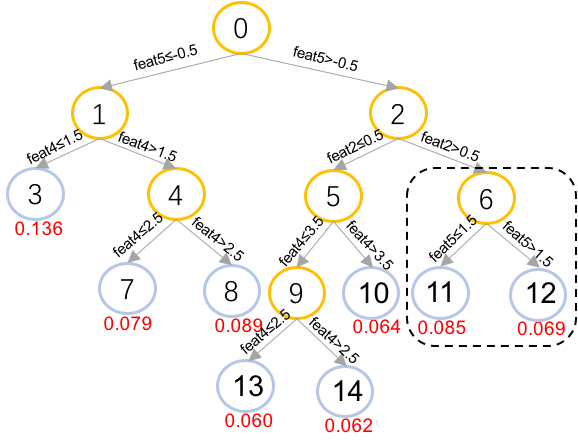
\includegraphics[width=0.45\textwidth]{pic/gbdttree.png}
 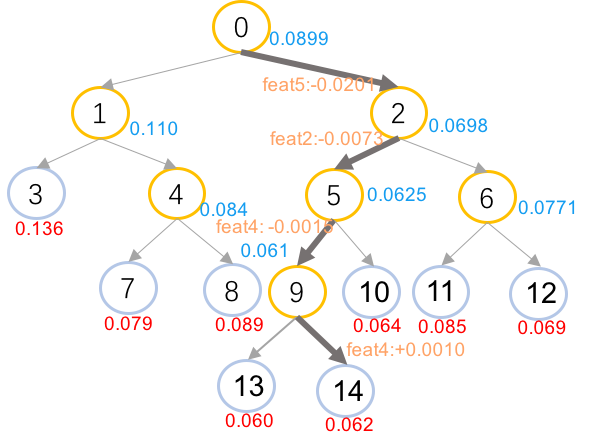
\includegraphics[width=0.45\textwidth]{pic/gbdtfc.png}
   \caption{Feature Contribution Example for GBDT}\label{figgbdt}
\end{figure}

By the propagation strategy, the average score is assigned to the node 6 which assumes  an instance 
falls into the left branch or the right with equal probability. So the expectation of intermediate nodes could be revised 
as in equation \ref{avgmod}:
\begin{equation}  \label{avgmod}
S_{p}=\frac{1}{2}(S_{c1}+S_{c2})\rightarrow\frac{N_{c1}\times S_{c1}+N_{c2}\times S_{c2}}{N_{c1}+N_{c2}},
\end{equation}  
where the $N_{c1}$ and $N_{c2}$ is the number of the instances fall into child nodes node c1 and c2.
These statistics need extra information from training process.

By viewing the computation in this brand new way, 
we get a  flexible interpretation mechanism by only using the leaf
node scores and instance distributions, regardless of the implement settings of GBDT.  Under the setting of
the LS loss function, we can see that not only the label distribution meets the 
prediction score on leaf node but the
label distribution of the intermediate node also meets our back propagated score. 
That is to say, the label distribution
method is a special case of our mechanism with this particular setting. Furthermore,
this method also supports the multiple classification problems.

